\documentclass[12pt]{article}
\usepackage{amsmath}
\usepackage{lipsum}
\usepackage{tikz}
\usetikzlibrary{shapes,backgrounds}
\usepackage{graphicx}
\graphicspath{ {img/} }
\begin{document}
\author{Zhexin Jia}
\title{CIS 425 Assignment 6}
\maketitle
\begin{enumerate}
\item[1.] Mitchell, Exercise 5.5
\item[(a)] ML code wrote In Assignment6.sml
\item[(b)] Explain your definition of reduce in one or two sentences.\\
Reduce function takes two parameter, a operation function and a tree.\\
It return the int number if the tree is a single LEAF; else recursively run oper (reduce oper tree, reduce oper tree) until reache the LEAF of the tree.\\
\item[2.] Mitchell, Exercise 5.6
\item[(a)] ML code wrote in Assignment6.sml
\item[(b)] Function Curry takes a function $f:('a * 'b)\to 'c$ as parameter and return a curried function $'a\to('b\to'c)$ which is the format of g.\\
Function UnCurry takes a function $g: 'a\to('b\to'c)$ as parameter and return a UnCurried function $('a * 'b)\to'c$ which is the format of f.\\
So the transformation for UnCurry(Curry(f)) is $UnCurry(Curry(f)) \to UnCurry(g) \to f$\\
The transformation for Curry(UnCurry(g)) is $Curry(UnCurry(g))\to Curry(f) \to g$
\item[3.] Mitchell, Exercise 5.7
\item[(a)]x.i is decleared to be an int, so the expression x.i interprets and returns an integer regardless of what was stored to x. So it is well typed for a compiler.\\
The Addition may not work because The union type x stores different data types in same memory location, it is either an int or char, when x is evaluated, the variable s is a pointer to a string value, but it would be interpreted as an integer because x.i returns an int. \\
The run-time system will not catch the problem.
\item[(b)]The same bug won't occur in this program. The run-time system will catch the problem.\\
Warning message: uncaught exception [Bind nonexhaustive binding failure] or similiar "match nonexhaustive" warnings. The $tag\_int$ doesn't povide a pattern math to $tag\_str$, the error message helps developer to consider all the possible data types in the domain.
\item[4.] Mitchell, Exercise 5.8, part (a) and part (b) only\\
ML code for part (a) and part (b) wrote in Assignment6.sml
\item[5.] Mitchell, Exercise 6.2\\
Type of sort function: $(('a *'a) \to bool) * 'a$ list $\to 'a$ list\\
Type of insert function: $(('a * 'a)$ list) $\to 'a$ list\\
Sort takes two arguments: less and list. Less is the function takes 2 parameters: element from the list and the list; less return a bool, so the type for less is $'a * 'a$ list $\to$ bool, the type for list is $'a$ list since we don't know the type of the list. So the parameters of the sort function is $(('a *'a) \to bool) * 'a$ list \\
Sort returns the function insert. \\
Insert takes two arguments: an element and a list. Insert returns a list. So the type of insert is $('a * 'a$ list) $\to 'a$ list. Since insert returns $'a$ list, Sort function returns $'a$ list too.\\
Thus, type of sort is $(('a *'a) \to bool) * 'a$ list $\to 'a$ list
\item[6.] Mitchell, Exercise 6.5\\
$(('a \to int)* 'a) \to int$\\
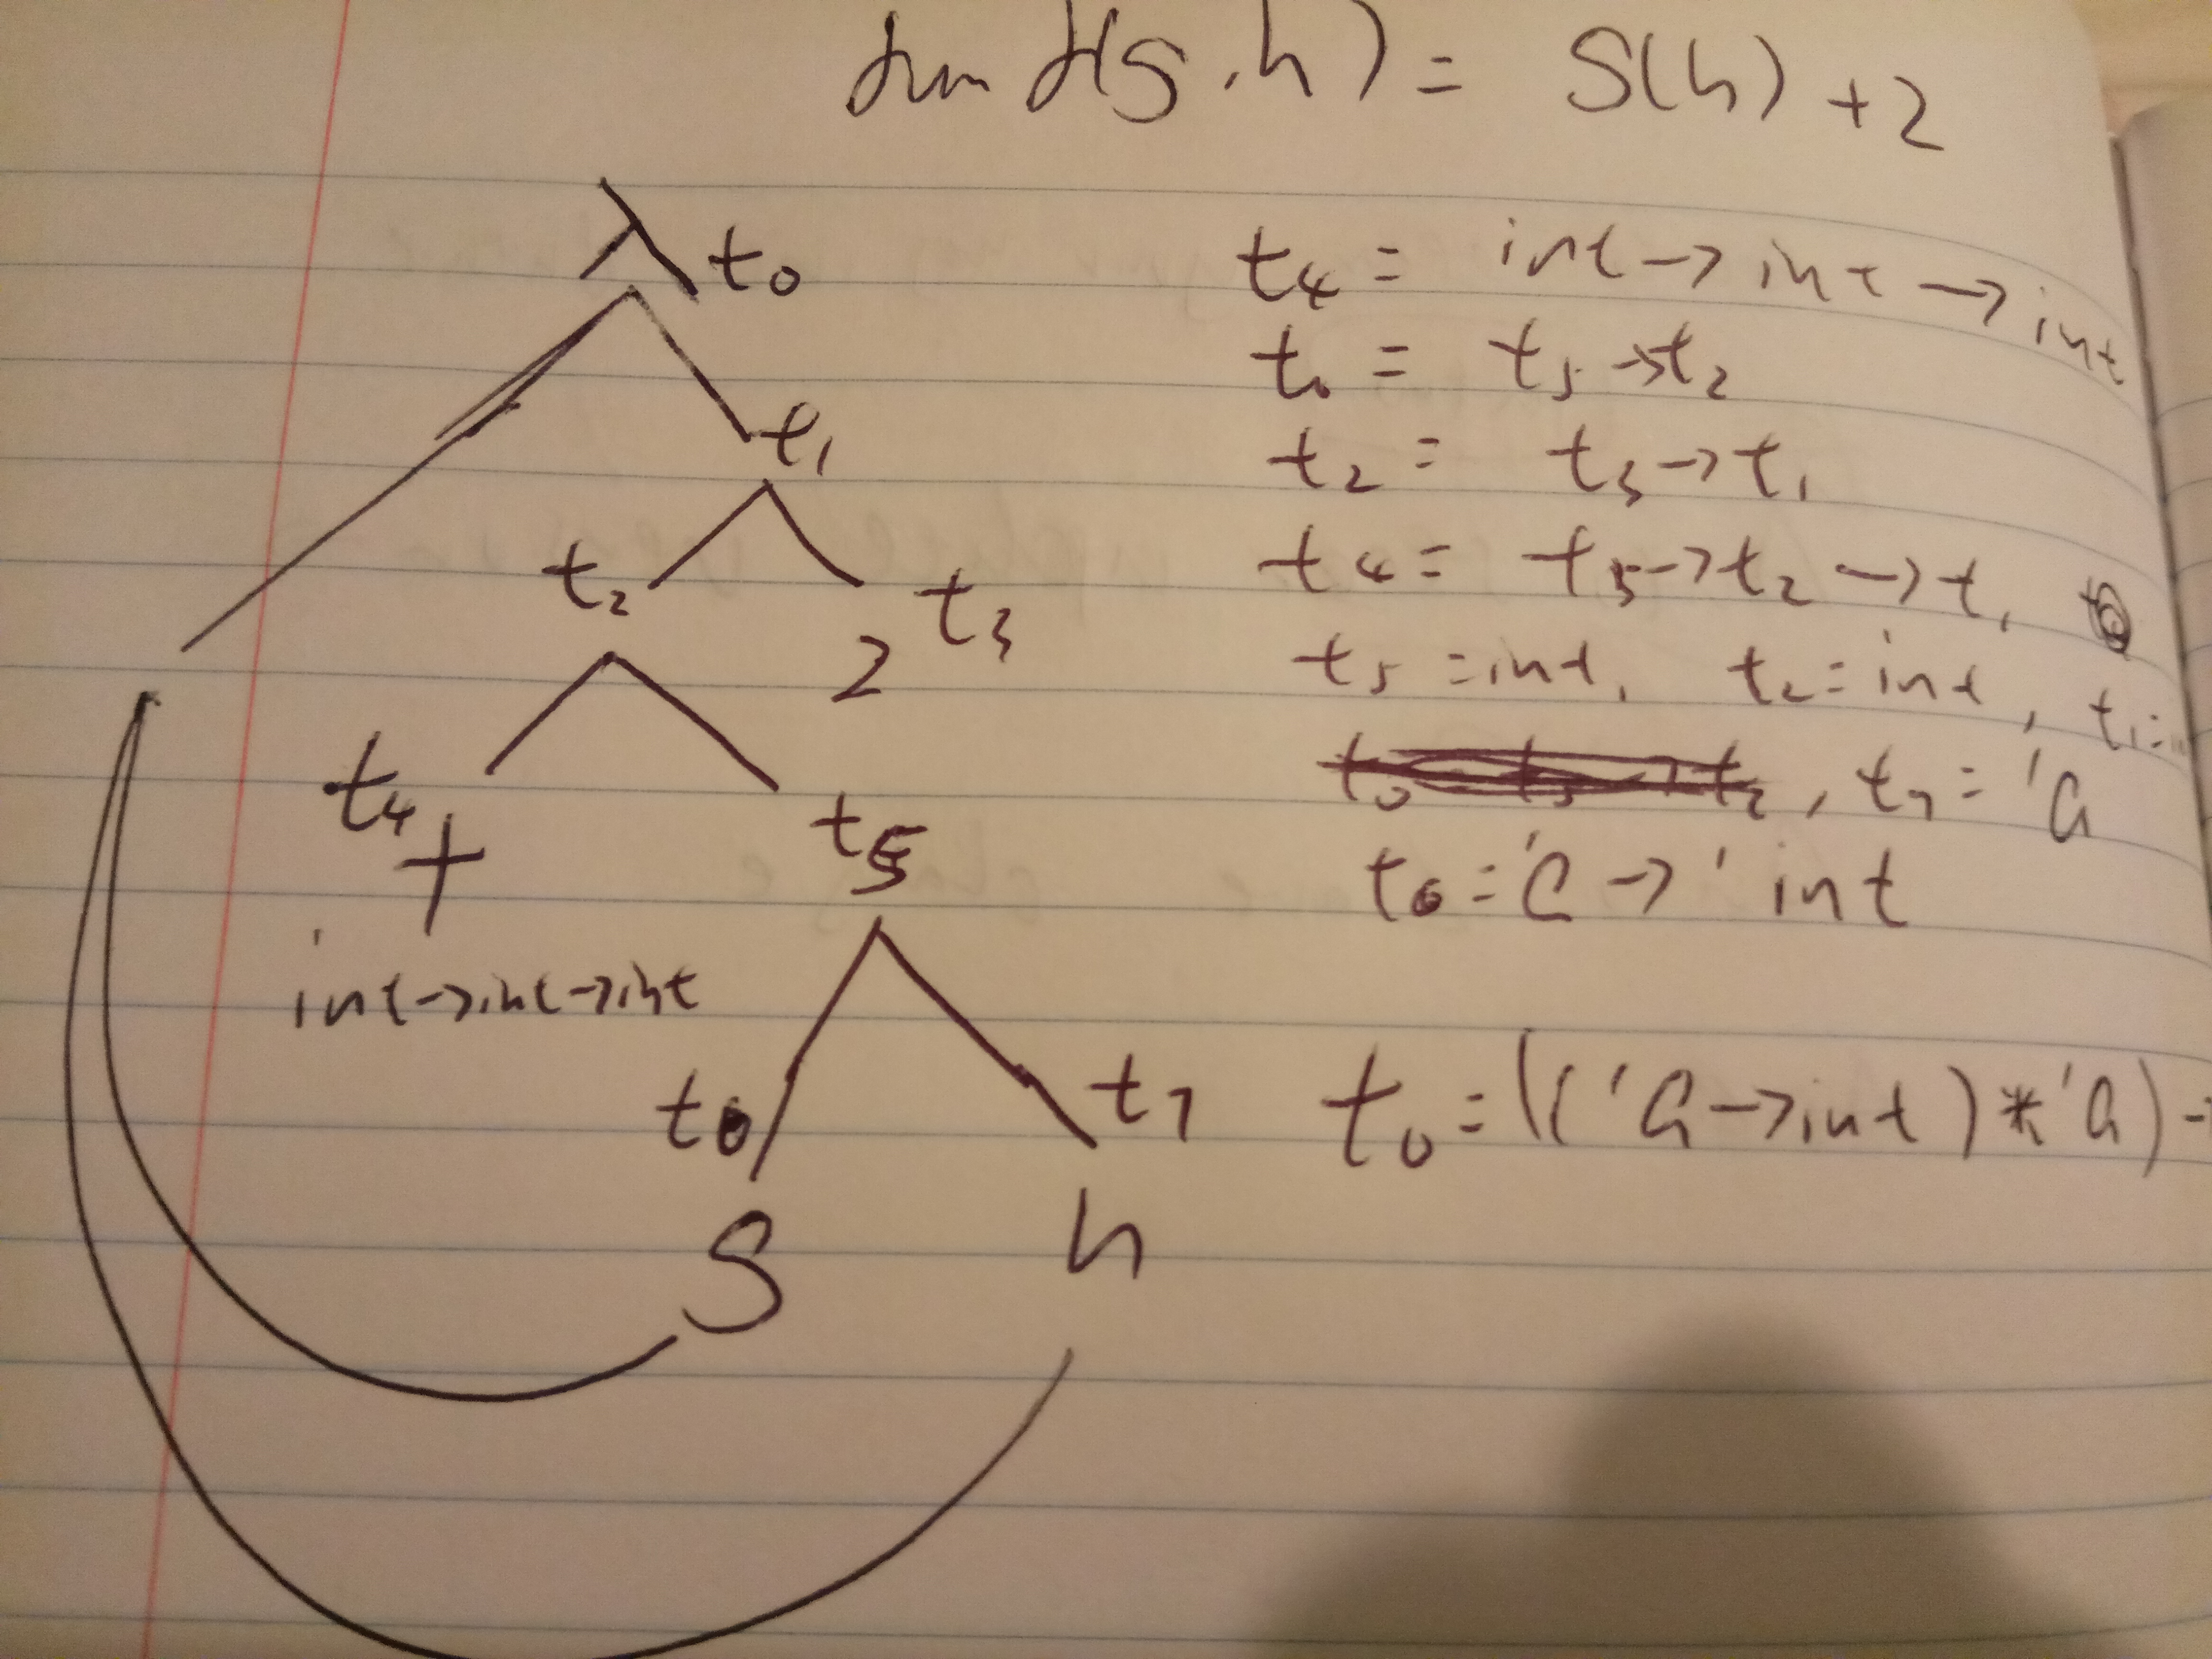
\includegraphics[width=\textwidth]{6.jpg}
\item[7.] Mitchell, Exercise 6.6\\
Output of the typechecker is error. The parse tree has a circular loop, it can't make the two g's have the same type.
\item[8.] Mitchell, Exercise 6.7\\
Type of append: $'a$ list * $'b \to 'b$\\
Why append has the type you give?\\
Append function taks two parameters, one list and one unknow type l/m, and returns l. There are no partern matching for the second argument, we can not decide the type of the second parameter. Since second parameter is 'l' and append returns 'l', the type of second parameter and type of return value is same.\\
How might knowing the type of this function help the programmer to find the bug?\\
The append function should take two lists as parameters, so their type should be same: $'a$ list, The function must returns a list since this function append one list onto another, so the return type is also $'a$ list, the correct type of this function should be: $'a$ list * $'a$ list $\to 'a$ list.\\
When we have the correct type of the function, programmre can easily find the bug from the wrong typed version since the function works with lists containsing items of the same type.
\end{enumerate}
\end{document}